\newif\ifresearch
\researchtrue % comment out to hide answers


\newif\iftwopage
\twopagetrue % comment this out to keep resume to two pages


\documentclass{article}
\pagenumbering{gobble}
\usepackage[raggedright]{titlesec}
\usepackage{etoolbox}
\usepackage{mfirstuc}	
\usepackage{hyperref}
\usepackage{titling}
\usepackage{amsmath}
\usepackage[margin=0.5in]{geometry}
\usepackage{array}
\usepackage{tabu}
\usepackage{multirow}
\usepackage{longtable}
\usepackage[utf8]{inputenc}
\usepackage{fancyhdr}
\usepackage{graphicx}
\usepackage{blindtext}
\usepackage{wrapfig}
\usepackage{enumitem}
\setlist{nosep}

\setlength{\arrayrulewidth}{0.05mm}

\titleformat{\section}[leftmargin]
{\raggedright\scshape\titlerule\vspace{0.5ex}}
{}
{0pt}
{}
\titlespacing*{\section}{2.8cm}{*1.8}{0.1cm}

\newcommand{\mygeometry}[1]{%
  \geometry{right=#1,left=\dimexpr#1+20mm\relax}
}
\mygeometry{15mm}

\titleformat{\subsubsection}[runin]
{\vspace{0.5ex}}
{$\bullet$}
{0.5em}
{}

\titlespacing{\subsubsection}
{0em}{0.1em}{1em}

\hypersetup{
    colorlinks=true,
    linkcolor=blue,
    filecolor=magenta,      
    urlcolor=cyan,
}
 
\urlstyle{same}

\title{Resume}
\date{2017-06-17}
\author{Abhishek Vaid}	

\begin{document}
\begin{huge} 
	\noindent Abhishek Vaid \hspace{1ex}
\end{huge} \href{http://linkedin.com/in/vaidabhishek86}{
\includegraphics[height=4ex]{linkedin}}
\\
\noindent \href{mailto: vaid.abhi@gmail.com}{vaid.abhi@gmail.com} \\+91 9886052252\\   
\vspace{-95pt}
\begin{flushright}
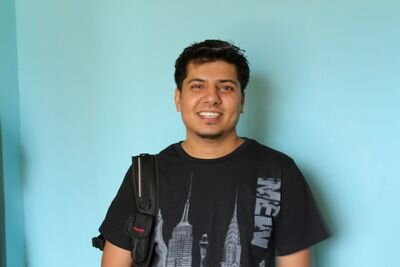
\includegraphics[width=2.8cm]{vaid}
\end{flushright}
 \vspace{-15pt}
\section{Profile}

\ifresearch
An entrepreneur who is passionate about intersection of \textbf{Technology, Software and Product}. I have \textbf{10+ years of experience} in building products across multiple verticals. I am currently working as \textbf{Principal Engineer} at \href{https://www.prophecy.io}{Prophecy.io}. In my previous stints, I have assumed role of \textbf{Technical Co-Founder} - \href{https://frrole.ai/}{frrole.ai}, \textbf{Engineering Manager / Technical Architect} at \href{https://www.urbancompany.com/delhi-ncr}{UrbanCompany} and \textbf{Lecturer (Computer Science)} at \href{lpu.in}{LPU}. In these roles, I have lead, managed and mentored teams of varied sizes. I also have extensive hands-on experience and deep interest in disciplines like \textbf{Large scale Data Engineering, Enterprise Software, Machine Learning, Data Science and Micro-service based Software architectures}. During my post-grad, I have contributed to several academic projects and authored several research papers. I am also extremely active on several MOOC platforms like \textbf{edX, Coursera, Udacity, Udemy, educative, cognitiveclass.ai, DataCamp}. Statistically speaking, I spend anywhere between \textbf{10 to 15 hours per week} on these platforms to learn new technologies. I strongly believe in continuous and self-driven growth.
\else

A post-graduate engineer, computer science enthusiast and a startup guy.  

\fi

\section{Education}
\begin{itemize}[leftmargin=-0.1ex]\setlength\itemsep{0.25em}\vspace{-10pt}
  \item[]  \href{http://iiitm.ac.in}{Indian Institute of Information Technology and Management (IIITM), Gwalior} \hfill Madhya Pradesh, India
  \item[] \textbf{5 Year Integrated Post Graduation in Information Technology} (CGPA: \textbf{8.34 /10}) \hfill 2004--2009
\end{itemize}\vspace{-3pt}

\section{Interests}
\begin{itemize}[leftmargin=-0.1ex]\setlength\itemsep{0.25em}\vspace{-10pt}
  \item Large Scale Data Engineering Pipelines and Data Science Frameworks. 
  \item Distributed Software Design, Reactive Architectures and Design Patterns
  \item Machine Learning, NLP, Text Mining
  \item Algorithm Design and Data Structures
  \item Software Frameworks, Database Modeling and API Design
\end{itemize}\vspace{-3pt}

\section{Hands-On Skills }
\begin{itemize}[leftmargin=-0.1ex]\setlength\itemsep{0.25em}\vspace{-10pt}
  \item \textbf{Programming languages}: Python, Java, Scala, Javascript, Typescript, C++, GoLang
  \item \textbf{API Toolkits}: Akka, NodeJs, Spring Boot, Flask, Django, Play, GRPC, Swagger
  \item \textbf{Distributed Processing Frameworks}: Storm, Spark, Hadoop, Airflow
  \item \textbf{Datascience / ML Toolkits}: PyTorch, TensorFlow, sklearn, Pandas
  \item \textbf{Databases}: MongoDB, ElasticSearch, MySQL, PostgreSql, Redis
  \item \textbf{Infrastrucure}: Docker, Kubernetes, AWS, GCP, Azure
\end{itemize}\vspace{-3pt}
  
\section{Work Profile}

\begin{itemize}[leftmargin=-1ex] \setlength\itemsep{0.25em}\vspace{5pt}

  \item[11/20' – 01/22'] \href{https://app.prophecy.io/}{\textbf{Prophecy.io}} \textbf{Principal Engineer}\hfill Gurugram, India (Remote)
	
	\item[]  \textbf{Prophecy.io} --- Prophecy.io is an SF based startup that offers low code Data Engineering for Spark \& Airflow and is used by top Enterprises. At Prophecy, I headed the Metadata team and was responsible for backend design, execution, delivery and support of key product features and engineering quality. I also spent a lot of time in actively coding and testing these features. Two of my most notable projects are listed below.  \vspace{5pt}
	\begin{itemize} \setlength\itemsep{0.5em}
		\item {\textbf{Lineage, Catalog \& Code Search}}  - Designed and implemented the entire Search infrastructure for Prophecy.io core product offering. This was a project with complex product specs where a versioned solution was vital to the success of search functionality. The implementation powers some of the key areas of Prophecy's overall product value like Lineage Search, Expression \& Symbol search, Full-text search on Scala / Python code files, Search on Entities and their Aspects (Avro schema backed JSONs). 
		\item {\textbf{Metadata 2.0 - Versioned Entity Graph}} - Implemented the \textbf{Metadata 2.0} service. This revision was a complete overhaul of earlier Metadata offering and required the implementation of an advance multi-fork two way Git Sync support, Event generation / consumption across micro-services over Kafka and publishing of an sdk (pbt - prophecy build tool) as a standalone module to manipulate entire Metadata entity graph, directly as a part of Git backed files within project repositories. The project also involved productization of advance git functionality like - interactive rebase, squash commits, parallel writes across branches and more. A new GraphQL API was also enabled to make it easy for clients to integrate.
		
	\end{itemize}\vspace{5pt}
	
	\item[09/17' – 11/20'] \href{https://urbanclap.com/}{\textbf{UrbanCompany}} \textbf{Technical Architect / Engineering Manager}\hfill Gurugram, India
	
	\item[]  \textbf{Urban Company} --- Urban Company (UC) is a Gurugram (India) based startup currently disrupting and redefining the online home services domain. Currently, UC is the market leader in India and has presence is 4 more countries. At UC, I own the backend engineering for Consumer Growth. My core responsibility includes having to engage directly with product and engineering VPs to define, plan and execute product and engineering roadmap. During this time, I've also written a lot of systems myself and managed teams of various sizes. \vspace{5pt}

	\begin{itemize} \setlength\itemsep{0.5em}
		
		\item {\textbf{Catalog Revamp 2020 and Search 2.0}} - Architected, Designed and delivered on two of the most important projects of 2020 in Growth Engineering. Both Catalog Revamp 2020 and Search 2.0 proved to be significant in removing technical debt and helped optimize for modern request funnels and App flows across various clients. Both these features brought significant uptake to conversion funnels.
		\item {\textbf{Logging and ELK Stack}} - Architected and implemented Elastic Stack and Logging Funnel. The system consumed 100(GB )/day of system and event logs from 30+ micro-services. 		
		\item {\textbf{Core SEO micro-service}} - Designed and implemented a new API stack to power UC's SEO use-case. Because of this effort, UC enjoyed top positions in 1st page search results (in top 3) for most of the competitive categories in the business.  
		\item {\textbf{Delivery and Pricing  Engine}} - Architected and implemented a service that powers pricing logic throughout the platform. This includes very complex categories like Packers \& Movers and Painters.
		\item {\textbf{Surge and Advance Payment}} - Designed and Implemented Surge and Advance Payment construct on our consumer app.
		\item \textbf{UC Homes/Weddings Content-Portal} - A content-heavy and SEO friendly, service discovery platform. \\ I handled the end-to-end execution of this project from start to end. 
		\item {\textbf{Refactoring}} - As the only architect at UC (at joining), I took key refactoring projects to kill technical debt and implement our internal micro-service framework.
	\end{itemize}\vspace{5pt}
	
  \item[12/12' – 07/17'] \href{https://frrole.ai/}{\textbf{Frrole AI:}} \textbf{Co-founder and CTO}\hfill Bengaluru, India
  \item[]  \textbf{Frrole AI} --- A Bangalore based \textbf{global AI Start-Up} that is redefining consumer intelligence by deploying best-in-class \textbf{AI and Machine Learning technologies to real-time large-scale social datasets from multiple networks}. I was involved in defining and shaping all aspects of Frrole ranging from \textbf{software architecture to design, development and scaling of our technical infrastructure}. I was also responsible for hiring and setting up our core team. 
  
Few notes on projects that I worked on:  \vspace{5pt}
  
  	\begin{itemize} \setlength\itemsep{0.5em}
    
    \item \href{https://frrole.ai/deepsense}{Frrole DeepSense (HumanticAi)} - An innovative and novel offering that \textbf{builds the personality profile and preference models of a potential customer based on their publicly available social footprint}. The platform also engineers predictive attributes about a person's behavior, needs, demographics and possible choices.
  
 	\item \href{https://frrole.ai/platform}{Frrole Consumer Intelligence Platform} - A suite of business-ready intelligence applications comprising of \href{http://api.frrole.com/}{Frrole Intelligence APIs} and \href{https://frrole.ai/scout}{Frrole Scout}. The product processes over 50 million data points every day in real-time to provide live api feed to over 30+ clients. The platform also provides historical access to over several TB of curated data. 
  
  	\item \textbf{Frrole News} - An \textbf{autonomous news aggregation engine} powered by real-time analysis of social data streamed from Twitter at a large scale. I designed, developed and scaled the core backend data models, APIs and intelligence layer. 
  	
	\end{itemize}
     
   \item[08/09' – 04/12'] \textbf{Head-Coordinator} and \textbf{Lecturer} at LPU \hfill Jalandhar, India
   
   \item[] I was responsible for managing the entire department comprising of \textbf{28 faculty members and 500 enrolled students}. I was directly responsible for \textbf{teaching quality}, \textbf{curriculum design}, and \textbf{pedagogical innovations}. I also \textbf{designed} and \textbf{instructed courses} on subjects like Data Mining, Distributed Systems, Data Structures, Linux, OOPS, Multimedia Communication, Java Programming, and Algorithms.

\end{itemize}

\begin{itemize}[leftmargin=-1ex] \setlength\itemsep{0.25em}
    \item[05/12' – 12/12'] \textbf{Learning Break} \hfill New Delhi, India
   \item[] Took a study break to augment my knowledge and enhance my skill set by pursuing relevant coursework (MOOC- Massively Open Online Courses) on platforms like \textbf{Coursera}, \textbf{edX}, and \textbf{Udacity}. Overall, I completed \textbf{~30 certified courses} in 8 months.
%  \item[05/08' – 07/08'] \textbf{Summer Intern at Sunworks Consultants Pvt. Ltd.} \hfill Gurugram, India
%   \item[] Conducted preliminary analysis in the field of Threat Assessment and Risk Evaluation, followed by the development of algorithms and strategies to fuel an Autonomous System for Threat Assessment and Evaluation.
\end{itemize}

%\section{Projects}
%\begin{itemize}[leftmargin=-1ex]\setlength\itemsep{0.25em}\vspace{5pt}
%   \item[08/08' – 08/09'] Master Thesis  --- \textbf{``Performance Analysis of Novel Evolutionary Algorithm Operators: An Implementation On Bounded Diameter Spanning Tree %Problem''}. The research results were subsequently published in Proceedings of International Conference on Contemporary Computing.
 %   \item[01/09' – 06/09'] \textbf{``Knowledge Discovery in Databases Using Evolutionary Algorithms''}, to understand the strengths \& weaknesses of using Multi-Objective Evolutionary Algorithms to solve association rule mining problems.
%   \item[07/08' – 08/08']  Developed an AI technique based on \textbf{Self Organizing Feature Maps} to automate the task of question selection in generating automatic online Question Paper Sets for various competitive examinations.
  %\item[05/07' – 08/07'] Bachelor's Thesis --- Developed \textbf{``FePAT - Fuzzy enabled Personality Assessment Technique''},  a  framework to maintain large-scale personality inventories for web applications. The whole framework and its core model were \textbf{tested with real world data} collected using custom made Fuzzy Based Questionnaire. 
   %\item[07/07' – 04/08'] Worked to mine out important \textbf{Multi-Dimensional Association Rules} from an \textbf{Environmental Dataset} of over 4 million records collected from over 30 sites in India. Algorithms were coded in Java.
%\end{itemize}

\section{Few Publications}
\begin{itemize}[leftmargin=-1ex]\setlength\itemsep{0.25em}\vspace{-10pt}
\item \textbf{``Association Rule Mining Using Multi-objective Genetic Algorithms: Strengths and Challenges''} presented at World Congress on Nature and Biologically Inspired Computing, 2009, Coimbatore. 
\item \textbf{``Multidimensional Association Rules from Large Weather Data Set: A Proposed Methodology''} accepted in Proceedings of International Conference on  Data Mining (DMIN), 2008, Las Vegas, USA. 
\item \textbf{``Automated Question Selection for Online Tests: A Novel Approach''} presented at International Congress on Pervasive Computing \& Management, 2008, New Delhi, India. 
%\item \textbf{``A Fuzzy enabled Personality Assessment Technique: FePAT''} presented at International Conference on Statistics and its Applications in Management (ICSAIM), 2008,  IIM Kozhikode, India.
%\item Paper based on my Master's Thesis: \textbf{``Property Analysis and Enhancement in Recombination Operator of Edge-Set Encoding for Spanning Tree Problem''}  presented at International Conference on Contemporary Computing (IC3),  2011, Noida, India.\label{masterthesis}
\end{itemize}

\end{document}